%results & evaluation, explicitly mentioning of known limitations

So far, we are able to generate Voronoi diagrams based on hex or random point selectors and visualise these diagrams.

Figure~\ref{fig:voronoi-random} shows the visualisation of a Voronoi diagram based on the random point selector.

\begin{figure}[H]
	\centering
	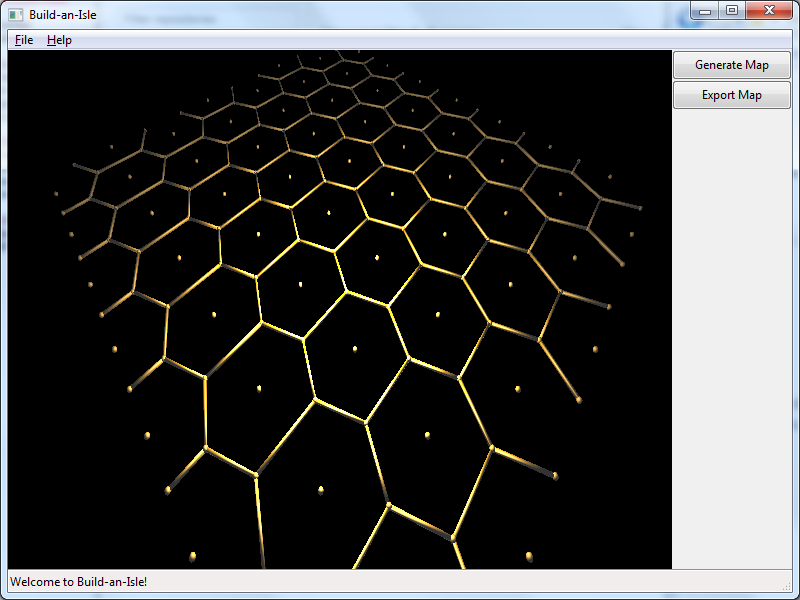
\includegraphics[width=\linewidth]{voronoi-hex}
	\caption{Visualisation of Voronoi diagram based on the hexagon point selector}
	\label{fig:voronoi-hex}
\end{figure}

Figure~\ref{fig:voronoi-hex} shows the visualisation of a Voronoi diagram based on the hexagon point selector.

